
\documentclass[xcolor={dvipsnames}]{beamer}
\usepackage{amsmath,amsfonts,amssymb,pxfonts,eulervm,xspace}
\usepackage{graphicx}
 \usepackage{multimedia}
\usepackage{media9}
\usepackage{minted}
\usepackage{mathtools}

\usepackage{animate}

\graphicspath{{./figures/}}
\usetheme{ccnycrest}


\begin{document}

\title{ CS102: File Input/Output}
\author{Hannah Aizenman}
\date{haizenm00@ccny.cuny.edu}


\begin{frame}
	\titlepage
\end{frame}

\begin{frame}{Input Stream}
	\begin{figure}
		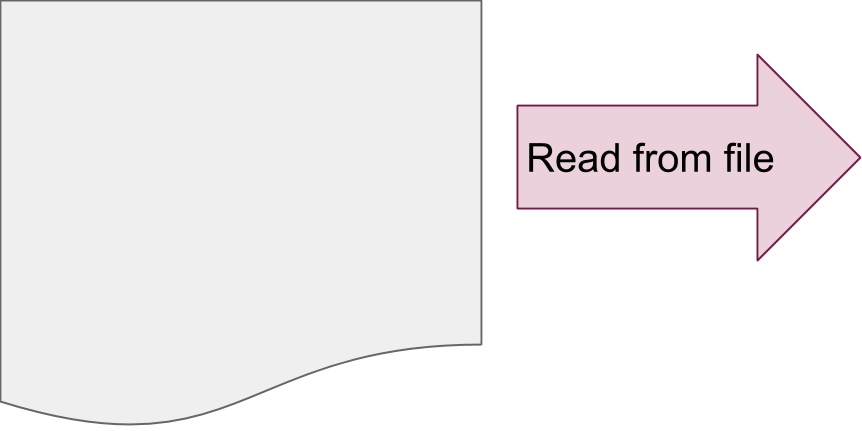
\includegraphics[width=1\textwidth]{read}
	\end{figure}
\end{frame}

\begin{frame}[fragile]{Opening and closing an input file}
\begin{minted}{c++}	
#include <iostream>
#include <fstream>
#include <string>
using namespace std;

int main(){
        string filename = "data.txt";
        ifstream inFile;
        inFile.open(filename.c_str());
        if (!inFile){
                //error handling
        }else{
                //process file
        }
        inFile.close();
        return 0;
}
\end{minted}
\end{frame}

\begin{frame}[fragile]{Reading contents of a file: Word by Word}
\begin{minted}{c++}
string filename = "inputword.txt";
string word;
ifstream inFile;
inFile.open(filename.c_str());
if (!inFile){
        cout<<"Error: Can't open "<<filename<<endl;
}else{
        while(inFile){
                inFile>>word;
                //do something with word variable
        }
}
inFile.close()
\end{minted}
\end{frame}

\begin{frame}{Reading contents of a file: Word by Word}
	\begin{figure}
		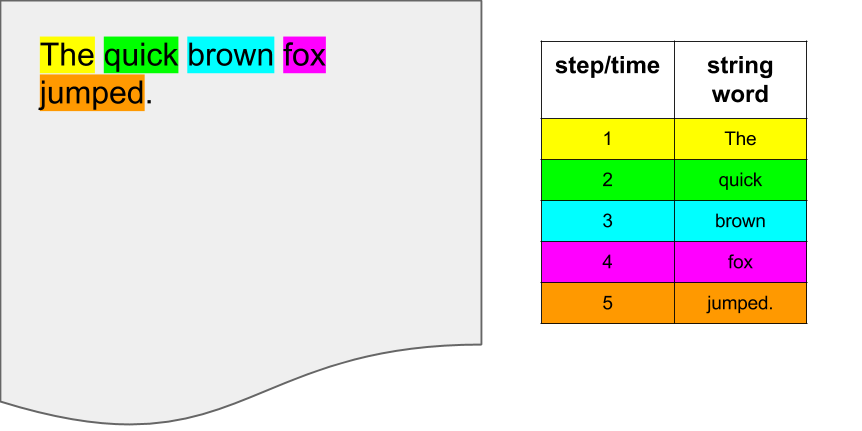
\includegraphics[width=1\textwidth]{readword}
	\end{figure}
\end{frame}


\begin{frame}[fragile]{Reading contents of a file: Numbers}
\begin{minted}{c++}
string filename = "inputnum.txt";
int number;
ifstream inFile;
inFile.open(filename.c_str());
if (!inFile){
        cout<<"Error: Can't open "<<filename<<endl;
}else{
        while(inFile){
                inFile>>number;
                //do something with number variable
        }
}
inFile.close();
\end{minted}
\end{frame}

\begin{frame}{Reading contents of a file: Numbers}
	\begin{figure}
		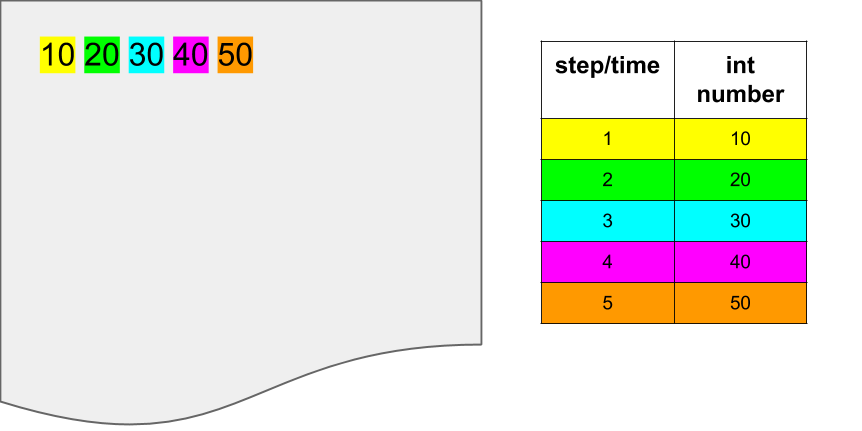
\includegraphics[width=1\textwidth]{readnumber}
	\end{figure}
\end{frame}

\begin{frame}[fragile]{Reading in data: Table}
\begin{minted}{c++}
string filename = "inputtab.txt";
string name;
int age;
ifstream inFile;
inFile.open(filename.c_str());
if (!inFile){
    cout<<"Error: Can't open "<<filename<<endl;
}else{
    while(inFile){
        inFile>>name>>age;
       //do something with name, age variables
    }
}
\end{minted}
\end{frame}

\begin{frame}{Reading in data: Table}
	\begin{figure}
		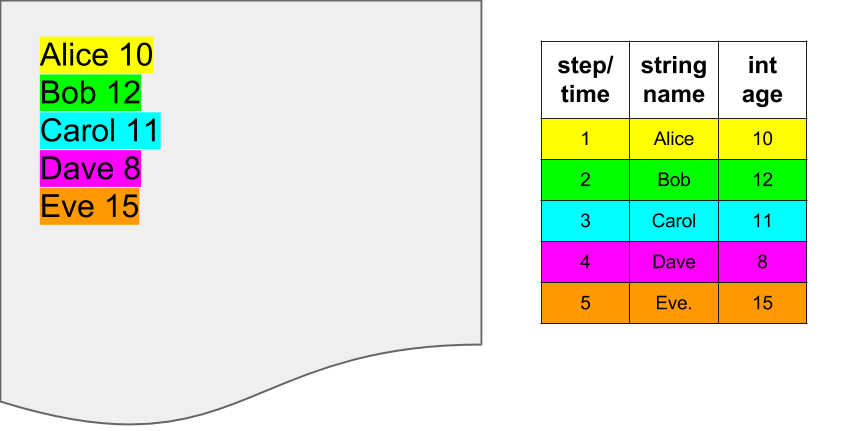
\includegraphics[width=1\textwidth]{readtable}
	\end{figure}
\end{frame}

\begin{frame}[fragile]{Reading in data: line by line}
\begin{minted}{c++}
string filename = "input.txt";
string line;
ifstream inFile;
inFile.open(filename.c_str());
if (!inFile){
    cout<<"Error: Can't open "<<filename<<endl;
}else{
    while(getline(inFile, line)){
        cout<<line<<endl;
       //do something with line variable
    }
}
inFile.close();
\end{minted}
\end{frame}

\begin{frame}{Reading in data: line by line}
	\begin{figure}
		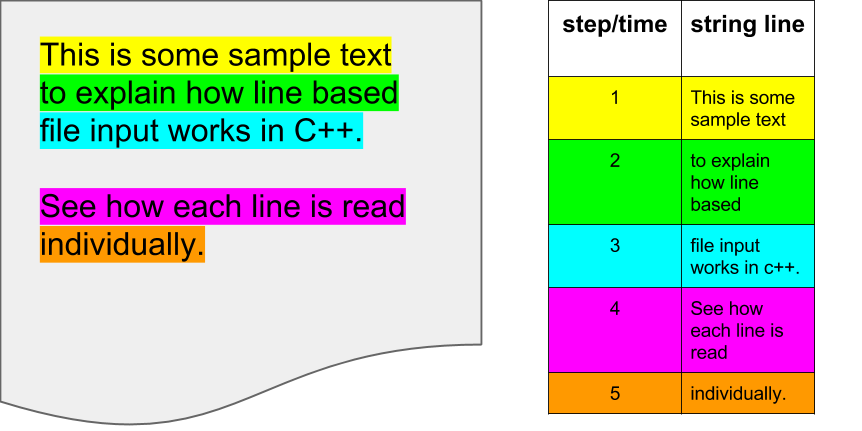
\includegraphics[width=1\textwidth]{readline}
	\end{figure}
\end{frame}

\begin{frame}{Output Stream}
	\begin{figure}
		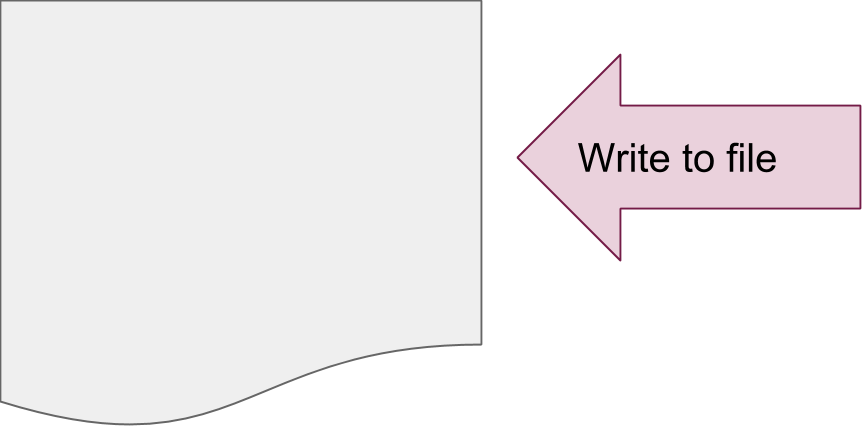
\includegraphics[width=1\textwidth]{write}
	\end{figure}
\end{frame}

\begin{frame}[fragile]{Writing out data}
\begin{minted}{c++}
string filename = "outfile.txt";
ofstream outFile;
outFile.open(filename.c_str());
outFile<<"This is text"<<endl;
outFile.close();
\end{minted}
\end{frame}

\begin{frame}{Writing out data: "outfile.txt"}
	\begin{figure}
		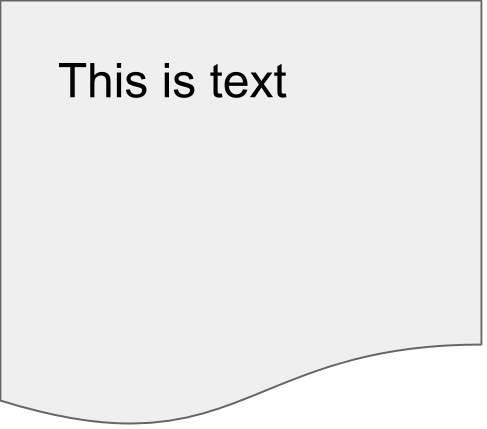
\includegraphics[width=.8\textwidth]{out}
	\end{figure}
\end{frame}

\begin{frame}[fragile]{Writing out more data}
\begin{minted}{c++}
string filename = "outfile.txt";
ofstream outFile;
outFile.open(filename.c_str());
outFile<<"This is text"<<endl;
outFile<<"This is some more text"<<endl;
outFile<<"This is even more text"<<endl;
outFile.close();
\end{minted}
\end{frame}


\begin{frame}{Writing out more data: "outfile.txt"}
	\begin{figure}
		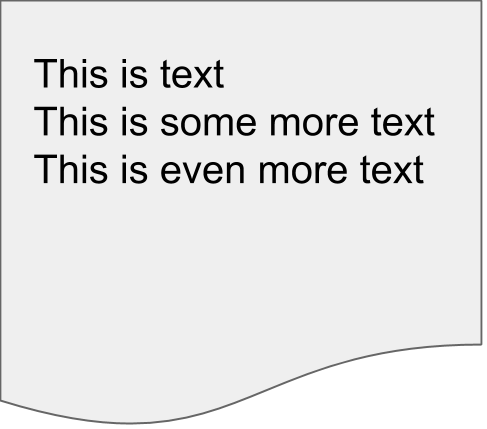
\includegraphics[width=.8\textwidth]{out2}
	\end{figure}
\end{frame}


\begin{frame}[fragile]{Writing out lots more data}
\begin{minted}{c++}
string filename = "outfile.txt";
ofstream outFile;
outFile.open(filename.c_str());
for (int i=0; i<100; i++){
    outFile<<"This is text"<<endl;
    outFile<<"This is some more text"<<endl;
    outFile<<"This is even more text"<<endl;
}
outFile.close();
\end{minted}
\end{frame}

\begin{frame}{Writing out lots more data: "outfile.txt"}
	\begin{figure}
		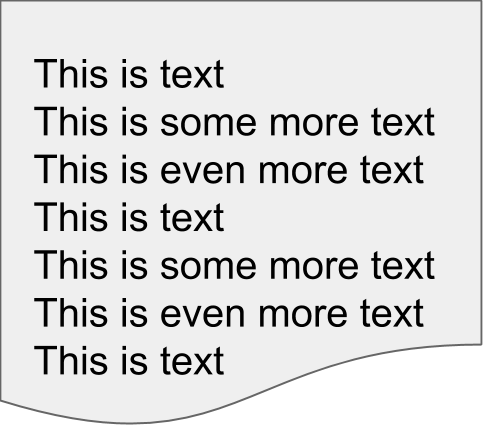
\includegraphics[width=.8\textwidth]{out3}
	\end{figure}
\end{frame}

\begin{frame}[fragile]{fstream file modes}
	\begin{center}
	\begin{minted}{c++}
		fileobject.open(filename, mode flag);
	\end{minted}
	\end{center}
\begin{table}
\begin{tabular}{|l|l|p{5cm}|}
	\hline
	\textbf{mode flag} & \textbf{mode} & {access}\\
	\hline
	ios::in & input & file open for reading \\
	\hline
	ios::out & output & file open for writing\\
	\hline
	ios::binary & binary & operations are performed in binary more (not text)\\
	\hline
	ios::ate & at end & output position starts at the end of the file \\
	\hline
	ios::app & append & ouput operations happen at end of the file (append to existing content)\\
	\hline
	ios::trunc & truncate & any contents in file are discarded before opening the file\\
	\hline
\end{tabular}
\end{table}
These flags can be combined with the bitwise OR operator (|).
\end{frame}

\begin{frame}{Random Access}
	\begin{block}{Read from a specific location in the file}
			\begin{itemize}
				\item input: inFile.seekg(offset, mode)
				\item output: outFile.seekp(offset, mode)
			\end{itemize}
		offset is the start position as measured in bytes from the file mode (either beginning, current, or end)
	\end{block}
	\begin{block}{Find the current position in the file}
			\begin{itemize}
				\item input: inFile.tellg()
				\item output: outFile.tellp()
			\end{itemize}
	\end{block}
	
\end{frame}
\end{document}

